\subsection{Spatiale filtrering}
Et spatialt filter er også kendt som: masks, kernels, templates eller windows. Et eksempel på et spatialt filter er vist på Figur~\ref{fig:spatial-filter}.\\

Der er en en-til-en sammenhæng mellem linear spatiale filtre og filtre i frekvensdomænet. Men spatiale filtre er i følge bogen mere alsidige end dem i frekvensdomænet, da de også kan bruges til ikke-linear filtrering. Hvilket ikke kan lade sig at gøre i frekvensdomænet.

\begin{figure}[H]
	\centering
	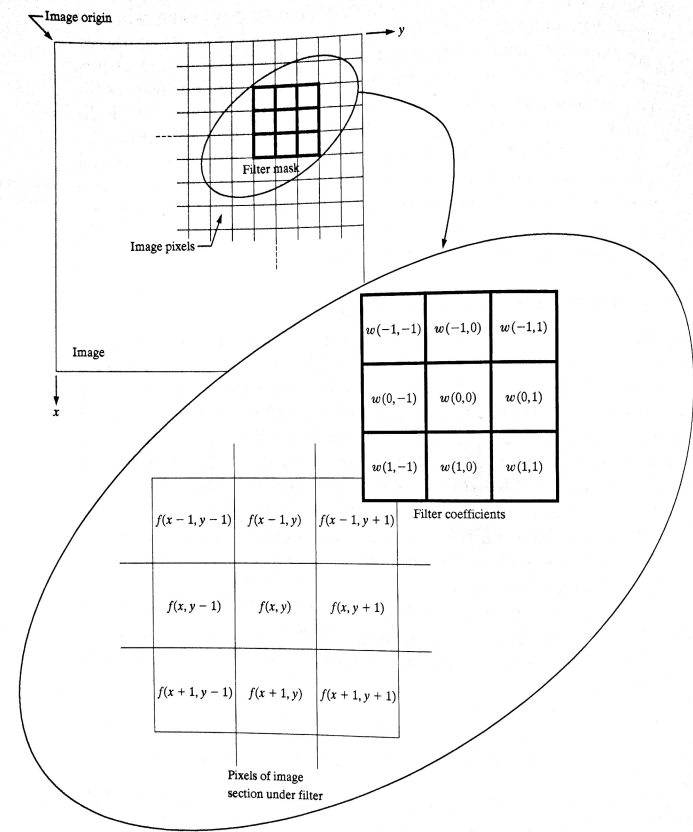
\includegraphics[width=0.8\linewidth]{figs/spm02/spatial-filter}
	\caption{Et 3 x 3 spatialt filter.}
	\label{fig:spatial-filter}
\end{figure}

\paragraph{Består af}

\begin{itemize}
	\item Et ''neighborhood'' og 
	\item En prædefineret operation.
\end{itemize}

Operationen er udført på de pixels der et i dette ''neighborhood''. Efter en operation er en ny pixel lavet i centeret af vores ''neighborhood''.